\section{Il modello di Attaccante Dolev-Yao}
\label{sec:dy}

In \cite{DY83}, gli autori hanno proposto un modello, noto anche come Dolev-Yao attacker model, per la formalizzazione degli attaccanti, questo modello viene comunemente utilizzato dai tool per la verifica formale dei protocolli basati sul modello simbolico, come vedremo con ProVerif e VerifPal.\\
Con questo tipo di modello si assume che l'attaccante sia in grado di:

\begin{itemize}
    \item intercettare, osservare ed eliminare i messaggi nella rete,
    \item costruire nuovi messaggi a partire da quelli osservati e iniettarli nella rete,
    \item disassemblare i messaggi non cifrati nelle parti che li compongono,
    \item iniettare nuovi messaggi nella rete costruiti con le informazioni di una sessione precendete del protocollo,
    \item decifrare messaggi cifrati solo se a conoscenza della chiave di cifratura.
\end{itemize}

\noindent L'attaccante di Dolev-Yao è un active attacker in grado di osservare, modificare ed eliminare i messaggi dalla rete, questo gli consente di utilizzare le regole descritte nella Figura \ref*{fig:rdy} per effettuare degli attacchi.\\
%L'attaccante Dolev-Yao è un attaccante che ha il pieno controllo della rete \fixnote{il DY \`e un active attacker}, può tentare ogni tipo di attacco possibile \fixnote{nope, pu\`o solo tentare quelli che gli vengono con le sue azioni.} grazie alla capacità di osservare, modificare ed eliminare i messaggi.\\
Nel modello Dolev-Yao si assume che la crittografia sia perfetta, ovvero che i meccanismi crittografici non siano vulnerabili, rendendo questo tipo di attaccante utile solo per attacchi alla logica dei protocolli.\\ 
%L'unica cosa che limita questo tipo di attaccante\fixnote{mr}{non userei limitato. Nel senso che il DY assume le primitive di encryption come blackbox, ma \`e anche limitato da tutte le azioni che non pu`\o fare. Per esempio, il social engineering non lo si pu\`o modellare, e nemmeno attacchi low level\ldots insomma credo sia buono per attacchi alla logica dei protocolli ma non di pi\`u} è l'assunzione della crittografia perfetta, ovvero l'assunzione per cui i meccanismi crittografici non sono vulnerabili, consentendo solo attacchi alla struttura del protocollo.\\
Grazie alle sue abilità, ai fini della verifica formale dei protocolli è utile identificare questo tipo di attaccante come la rete stessa.
%Questo tipo di attaccante è così potente\fixnote{non \`e una questione di potenza ma una scelta. Siccome ci fa comodo che l'attaccante venga identificato con la rete allora decidiamo che il DY lo sia. Questo rende l'attaccante molto forte} che è inutile differenziarlo dalla rete, si può dire che è la rete stessa.

\subsection{Primitive nel modello Dolev-Yao}
%\fix{mr}{forse \`e meglio citare il paper da cui hai preso il testo}
Considerando un attaccante attivo nel modello standard di Dolev e Yao, in grado di intercettare i messaggi, decifrarli solo se in possesso della chiave di decifratura, generarne di nuovi in base alla sua conoscenza e iniettarli nella rete immedesimando qualsiasi agente è possibile definire delle regole per il suo comportamento, come fatto in \cite{RVV17}. \\
Sia $\mathcal{S}$ un sistema e $\mathcal{S_{DY}}$ un sistema in presenza di attaccante del modello Dolev-Yao, sia IK un insieme di messaggi e DY(IK) il più piccolo insieme chiuso rispetto le regole del sistema  $\mathcal{S_{DY}}$ di generazione (G) e di analisi (A). \\
La regola G consente all'attaccante di generare nuovi messaggi a partire dai messaggi conosciuti, attraverso la concatenazione e utilizzando la crittografia simmetrica e asimmetrica, la regola A descrive come l'attaccante può decomporre i messaggi. 

\begin{figure}[h!]
    \centering
    \footnotesize
    \subfloat{\scalebox{0.85}{
    \begin{math}
    \infer[G_{assioma}]{M\in DY(IK)}{M\in IK}
    \end{math}
    }}
    \qquad
    \subfloat{\scalebox{0.85}{
    \begin{math}
        \infer[G_{concat}]{[M_1,M_2]\in DY(IK)}{M_1\in DY(IK) \quad M_2\in DY(IK)}
    \end{math}
    }}
    \\
    \subfloat{\scalebox{0.85}{
    \begin{math}
        \infer[G_{critA}]{\{M_1\}_{M_2}\in DY(IK)}{M_1\in DY(IK) \quad M_2\in DY(IK)}
    \end{math}
    }}
    \quad
    \subfloat{\scalebox{0.85}{
     \begin{math}
            \infer[G_{critS}]{\{|M_1|\}_{M_2}\in DY(IK)}{M_1\in DY(IK) \quad M_2\in DY(IK)}
    \end{math}
    }}
    \\
    \subfloat{\scalebox{0.85}{
    \begin{math}
        \infer[A_{concat_{i}}]{M_i\in DY(IK)}{[M_1,M_2]\in DY(IK)}
    \end{math}
    }}
    \quad
    \subfloat{\scalebox{0.85}{
    \begin{math}
        \infer[A_{critS}]{M_1\in DY(IK)}{\{|M_1|\}_{M_2}\in DY(IK) \quad M_2\in DY(IK)}
    \end{math}
    }}
    \\
    \subfloat{\scalebox{0.85}{
    \begin{math}
        \infer[A_{critA}]{M_1\in DY(IK)}{\{M_1\}_{M_2}\in DY(IK) \quad inv(M_2)\in DY(IK)}
    \end{math}
    }}
    \quad
    \subfloat{\scalebox{0.85}{
    \begin{math}
        \infer[A^{-1}_{critA}]{M_1\in DY(IK)}{\{M_1\}_{inv(M_2)}\in DY(IK) \quad M_2\in DY(IK)}
    \end{math}
    }}
    \caption{Sistema delle regole $\mathcal{S_{DY}}$ per l'attaccante Dolev-Yao}
    \label{fig:rdy}
\end{figure}

\newpage
\subsection{Le primitive nella modellazione UML}

Le primitive descritte nella Figura \ref{fig:rdy} vengono rappresentate anche nella modellazione del protocollo attraverso l'utilizzo dei diagrammi UML.\\
La primitiva $G_{concat}$ (concatenazione) appare nei diagrammi UML quando abbiamo più input in ingresso ad un oggetto con un singolo output, ad esempio viene utilizzata quando in un oggetto viene preparato un pacchetto, dati vari parametri in ingresso vengono concatenati prima di essere inoltrati.\\
Al contrario la primitiva $A_{concat}$ (deconcatenazione) appare quando abbiamo un singolo input e in uscita più output, come quando abbiamo in ingresso un pacchetto e dobbiamo ricavare qualche elemento da cui è composto.\\
\begin{figure}[h!] 
    \centering 
        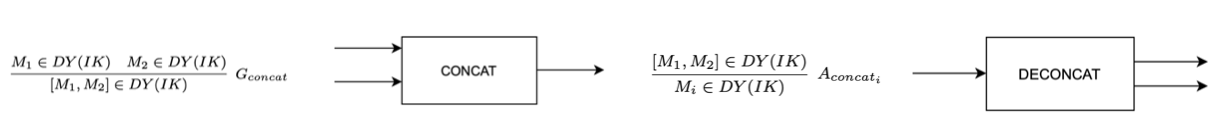
\includegraphics[width=\textwidth]{../img/1.png} 
        \caption{Concatenazione e deconcatenazione} 
\end{figure}\\
Nella modellazione UML gli oggetti di encryption e decryption sono considerati delle black box, questo perch\'e in caso di crittografia simmetrica corrispondono alle primitive $G_{critS}$ e $A_{critS}$ e in caso di crittografia asimmetrica corrispondono alle primitive $G_{crittA}$ e $A_{crittA}$ del modello Dolev-Yao.\\
\begin{figure}[h!] 
    \centering 
        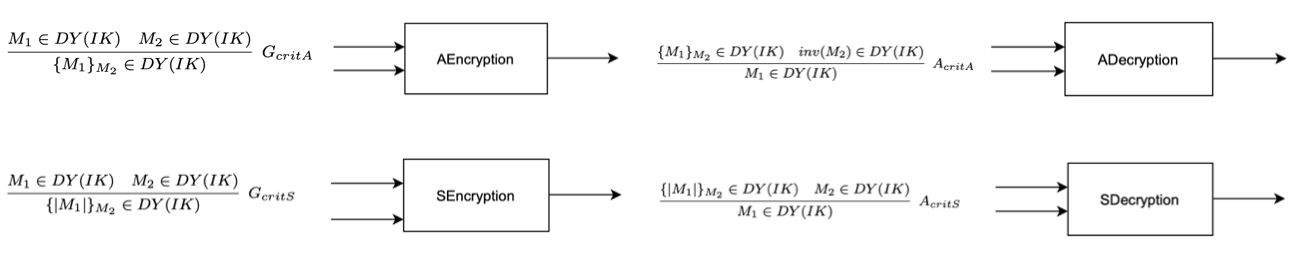
\includegraphics[width=\textwidth]{../img/2.png} 
        \caption{Encryption e decryption a chiave simmetrica e asimmetrica} 
\end{figure}\\
Nel caso in cui nel diagramma sia rappresentato un oggetto per la firma di un messaggio o per la verifica della firma, ancora una volta troviamo nel modello Dolev-Yao le primitive necessarie, ovvero la primitiva  $G_{crittA}$, la quale si occupa della firma di un messaggio prendendo come input la chiave privata e il messaggio, e la primitiva $A^{-1}_{crittA}$, la quale verifica la firma utilizzando la chiave pubblica.\\
\begin{figure}[h!] 
    \centering 
        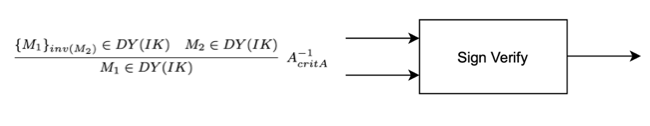
\includegraphics[width=0.6\textwidth]{../img/3.png} 
        \caption{Verifica della firma} 
\end{figure}\\
\begin{figure}[h!] 
    \centering 
        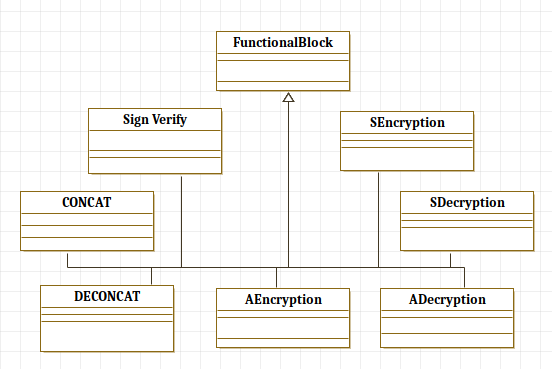
\includegraphics[width=0.8\textwidth]{../img/cd_1.png} 
        \caption{Diagramma delle classi delle primitive} 
\end{figure}\\




